\pdfoutput=1
\documentclass[11pt,a4paper]{article}

% ---------------------------------------------------------------------------
% Deciding D-stability is coNP-hard.
% Author metadata: set the three macros below before submission.
% ---------------------------------------------------------------------------
\newcommand{\PaperAuthor}{}
\newcommand{\PaperAffiliation}{}
\newcommand{\PaperDate}{September 2026}

\usepackage[T1]{fontenc}
\usepackage[utf8]{inputenc}
\usepackage{lmodern}
% Font expansion is off: with it, pdfTeX (MiKTeX 25.12) once placed a caption line 15220pt
% off the page (a layout-dependent Td offset).  build.py scans the PDF for such offsets.
\usepackage[expansion=false]{microtype}
\usepackage[a4paper,margin=1.05in]{geometry}
\usepackage{amsmath,amssymb,amsthm,mathtools}
\usepackage{booktabs}
\usepackage{array}
\usepackage{enumitem}
\usepackage{graphicx}
\usepackage{caption}
\captionsetup[table]{justification=raggedright,singlelinecheck=false}
\usepackage{xcolor}
\usepackage[hyphens,obeyspaces,spaces]{url}
\usepackage[colorlinks=true,linkcolor=blue!55!black,citecolor=blue!55!black,urlcolor=blue!55!black]{hyperref}
\hypersetup{pdftitle={Deciding D-stability is coNP-hard},
  pdfauthor={\PaperAuthor},
  pdfsubject={D-stability, computational complexity, Hurwitz stability},
  pdfkeywords={D-stability, diagonal scaling, coNP-hardness, subset sum, Pell equation, Routh-Hurwitz, Lean 4}}

\setlist{itemsep=2pt,topsep=3pt}
\setlength{\emergencystretch}{1.5em}

\theoremstyle{plain}
\newtheorem{theorem}{Theorem}[section]
\newtheorem{proposition}[theorem]{Proposition}
\newtheorem{lemma}[theorem]{Lemma}
\newtheorem{corollary}[theorem]{Corollary}
\newtheorem*{mainthm}{Theorem}
\theoremstyle{definition}
\newtheorem{definition}[theorem]{Definition}
\newtheorem{example}[theorem]{Example}
\theoremstyle{remark}
\newtheorem{remark}[theorem]{Remark}

\newcommand{\R}{\mathbb{R}}
\newcommand{\C}{\mathbb{C}}
\newcommand{\Q}{\mathbb{Q}}
\newcommand{\Z}{\mathbb{Z}}
\newcommand{\N}{\mathbb{N}}
\newcommand{\Real}{\operatorname{Re}}
\newcommand{\Imag}{\operatorname{Im}}
\newcommand{\diag}{\operatorname{diag}}
\newcommand{\one}{\mathbf{1}}
\newcommand{\cB}{\mathcal{B}}
\newcommand{\cU}{\mathcal{U}}
\newcommand{\cP}{\mathcal{P}}
\newcommand{\scl}[2]{#1^{(#2)}}
\newcommand{\be}{\mathbf{e}}
\newcommand{\prob}[1]{\textup{\textsc{#1}}}
\DeclareUrlCommand\lean{\urlstyle{tt}}
\def\UrlBreaks{\do\.\do\/\do\_\do\-}

\title{Deciding D-stability is coNP-hard}
\author{\PaperAuthor\\[2pt]\small\PaperAffiliation}
\date{\PaperDate}

\begin{document}
\maketitle

\begin{abstract}
A real square matrix $A$ is D-stable if $DA$ is Hurwitz for every positive
diagonal matrix $D$. Explicit criteria are known up to order three, and decision
procedures for order four. It has long been suggested that the general problem is
intractable, but to our knowledge no hardness proof has been available. We show that deciding
D-stability of a rational matrix is coNP-hard, and that deciding whether some
positive diagonal scaling has an eigenvalue in the open right half-plane is
NP-hard.

The reduction is from PARTITION. For weights $w_1,\dots,w_m$ it produces an
integer matrix of order $m+4$ with entries of polynomial bit length. The matrix is
D-stable if the weights admit no equal split, and has a strictly destabilizing
positive scaling otherwise. The hardness therefore holds for the promise problem
and for D-semistability as well. It is hardness in the weak sense (binary
encoding), since the entries grow like the fourth power of the total weight. The
hard matrices consist of a $4\times4$ core together with $m$ first-order
attachments at one coordinate.

The mechanism is a subset-sum obstruction. Fast attachments act as static load and
slow ones are invisible, so the matrix is destabilized exactly when a subset sum of
the loads lands in a window of loads at which the core is D-unstable. The window
must be exponentially narrow and yet exactly certified. We obtain it from a core
whose window is born at the irrational parameter $\sqrt3$, so that Pell
approximations $p/q$ of $\sqrt3$ give rational windows of width $\Theta(1/q)$. We
control every imaginary-axis contact by one polynomial inequality that places its
height under the window's semicircle.

The mathematical argument, including the explicit integer encoding, is formally
verified in Lean~4 with Mathlib. Only the complexity-theoretic packaging (running time and trivial instances) is
informal.
\end{abstract}

\noindent\textbf{Keywords:} D-stability; diagonal scaling; computational complexity;
coNP-hardness; subset sums; Pell equation; Routh--Hurwitz; formal verification.\\[2pt]
\textbf{MSC 2020:} 93D09, 15A18, 68Q17 (primary); 11D09, 93D20 (secondary).

\tableofcontents

% =========================================================================
\section{Introduction}\label{sec:intro}

A real $N\times N$ matrix $A$ is \emph{D-stable} if $DA$ is Hurwitz, that is, has all
eigenvalues in the open left half-plane, for every positive diagonal matrix $D$.
Equivalently, the linear system $\dot x=DAx$ is asymptotically stable whatever the
positive time scales of its coordinates. Since $DA$ and $AD=D^{-1}(DA)D$ are similar,
one may scale on either side; we use right scaling from Section~\ref{sec:prelim} on.

The notion goes back to Enthoven and Arrow~\cite{enthoven1956} and Arrow and
McManus~\cite{arrow1958} in the stability of competitive equilibria. It has since
become a standard object of matrix
theory~\cite{johnson1974,cross1978,hershkowitz1992,logofet1993,hornjohnson1991,kushel2019}.
Explicit criteria are classical for $N\le3$~\cite{cain1976}, and decision procedures
are known for $N=4$~\cite{kanovei1998,impram2005}. For general $N$ no explicit
criterion is known, and recent work develops hierarchies of sufficient
tests~\cite{kushel2019,kushel2026}.

Chen, Fan and Yu~\cite{chen1995} related D-stability to a real structured singular
value. They remarked that checking D-stability ``may in general be an NP-hard
problem''. The remark has been repeated since~\cite{giorgi2015}. Recent work describes
exact tests as computationally intractable for larger systems~\cite{kushel2026}, and
computational methods for D-stability as a largely open area~\cite{casasanta2026}. As
far as we are aware, no reduction has been given (Section~\ref{sec:discussion}).
The known hardness results for structured singular values~\cite{braatz1994}, for
interval matrices~\cite{poljak1993,nemirovskii1993} and for matrix
polytopes~\cite{gurvits2009} concern general matrices, interval families or convex
hulls. Hardness for general instances does not transfer to the special
matrices through which D-stability is expressed.

\paragraph{Main result.}
Let PARTITION be the NP-complete problem~\cite{karp1972,garey1979}: given
positive integers $w_1,\dots,w_m$, decide whether the index set splits into two parts
of equal weight. Matrices are encoded by their rational entries in binary.

\begin{mainthm}
There is a polynomial-time algorithm that maps every PARTITION instance
$w=(w_1,\dots,w_m)$ to an integer matrix $M(w)$ such that:
\begin{itemize}
\item if $w$ is a no-instance, then $M(w)$ is D-stable;
\item if $w$ is a yes-instance, then some positive diagonal scaling of $M(w)$ has an
eigenvalue with positive real part.
\end{itemize}
Consequently:
\begin{itemize}
\item deciding D-stability of a rational matrix is coNP-hard, and so is deciding
D-semistability;
\item deciding whether a rational matrix admits a destabilizing positive diagonal
scaling is NP-hard.
\end{itemize}
All three statements hold already for the promise problem that separates D-stable
matrices from strictly D-unstable ones. For nontrivial instances, $M(w)$ has order
$m+4$ and consists of a $4\times4$ core with $m$ first-order attachments at one
coordinate.
\end{mainthm}

The entries of $M(w)$ have magnitude $\Theta(T^4)$, where $2T=\sum_jw_j$. This is not
bounded by a polynomial in the input length, so the hardness is in the weak sense, for
binary encodings (Section~\ref{sec:discussion}).

\paragraph{The mechanism.}
The reduction uses \emph{star matrices}. A core $B$ interacts with $m$ scalar
attachments through one coordinate, the \emph{port}. Attachment $j$ relaxes toward the
port on its own time scale and feeds back with load $r_j$. An attachment much faster than
the port acts as a static load on the port's diagonal, and one much slower is invisible;
this is developed in a companion manuscript~\cite{companion2026}, and the facts needed
here are proved in Section~\ref{sec:prelim}. Hence, if the
core loaded statically by a subset sum $\sum_{j\in S}r_j$ is D-unstable, so is the star
matrix. If the set of D-unstable static loads is a window $\cU$, instability of the
star matrix looks like the question ``does some subset sum lie in $\cU$?''.

There are two obstacles to turning this into a reduction:
\begin{enumerate}[label=(\roman*)]
\item The window must be exponentially narrow compared with its distance from the
ends of the load range, since otherwise only boundedly many large pieces matter and
the subset question is easy. At the same time it must have exactly known, rational
position and width.
\item Avoiding the window must be \emph{sufficient} for D-stability. The attachments
of a fixed partition could still produce contacts, that is, imaginary-axis
eigenvalues, at intermediate time scales.
\end{enumerate}

\paragraph{How the obstacles are overcome.}
We use a $4\times4$ core whose principal minors are equal within each order and
type (inner coordinates versus minors containing the port). Its scaled characteristic
polynomial then depends on the three inner rates only through their elementary
symmetric functions. Its Routh--Hurwitz test can fail only through a single quadratic
$K(h)$ in the port's self-coefficient $h$ (Section~\ref{sec:core}).

In our one-parameter family $\rho$, the window $\{K<0\}$ is born at the irrational
point $\rho=\sqrt3$. Pell solutions $p^2-3q^2=1$ therefore give windows with rational
endpoints and width $\Theta(1/q)$, which settles~(i).

For~(ii) we prove one polynomial inequality. It shows that the normalized height of
every contact of the static core lies under the semicircle spanned by the window. The
total lag of the attachments, on the other hand, is at least the distance from their
effective static load to the nearest subset sum. Together these exclude all contacts.
A continuation in $\rho$ from a window-free core then gives D-stability.

The proof is self-contained. The safety theorem (Theorem~\ref{thm:safety}) is proved
here, and the stable direction uses only elimination, the elementary rounding bound of
Lemma~\ref{lem:rounding} and continuation. The companion paper~\cite{companion2026}
supplies motivation and a more general theory of star matrices, which the hardness
proof does not require.

\paragraph{Verification.}
The proofs of Sections~\ref{sec:prelim}--\ref{sec:encoding} are formally verified in
Lean~4~\cite{demoura2021} with Mathlib~\cite{mathlib2020}. The exceptions are
explicitly marked: Remarks~\ref{rem:schur} and~\ref{rem:control}, which are not used in
the proofs and are checked by exact computation, and Corollary~\ref{cor:complexity}. The formal
root is \lean{DStabilityHardness.partition_dichotomy}, which covers the explicit integer
encoding, its entry bounds, the logarithmic Pell search, and the promise form including
D-semistability. It depends only on the axioms \lean{propext}, \lean{Classical.choice}
and \lean{Quot.sound}. The polynomial certificates enter the formal proof as ring
identities and are checked by the kernel. Section~\ref{sec:verification} gives the
correspondence. What remains informal is the complexity-theoretic packaging in
Corollary~\ref{cor:complexity}: the running-time analysis and the handling of trivial
instances.

\paragraph{Organization.}
\begin{itemize}
\item Section~\ref{sec:prelim}: definitions, quartic Routh--Hurwitz facts, absorption
and the safety theorem.
\item Section~\ref{sec:core}: the core family, its window and the two certificates.
\item Section~\ref{sec:reduction}: the proof of the reduction.
\item Section~\ref{sec:encoding}: the integer encoding and complexity consequences.
\item Section~\ref{sec:example}: a worked example.
\item Section~\ref{sec:verification}: the formal verification.
\item Section~\ref{sec:discussion}: related work and open problems.
\end{itemize}

% =========================================================================
\section{Preliminaries}\label{sec:prelim}

\subsection{Scalings and decision problems}
For $A\in\R^{N\times N}$ and a rate vector $d\in(0,\infty)^N$ put
$\scl Ad=A\diag(d)$. It has the same eigenvalues as $\diag(d)A$. The matrix $A$ is:
\begin{itemize}
\item \emph{D-stable} if every $\scl Ad$ is Hurwitz;
\item \emph{strictly D-unstable} if some $\scl Ad$ has an eigenvalue with positive real part;
\item \emph{D-semistable} if it is not strictly D-unstable, that is, if no $\scl Ad$
with $d>0$ has an eigenvalue with positive real part.
\end{itemize}
D-stable matrices are D-semistable. All three notions are invariant under
multiplication of $A$ by a positive scalar $c$, since $\scl{(cA)}d=\scl A{cd}$. We use the
Hurwitz convention throughout; parts of the literature, e.g.~\cite{kushel2019},
state results for positive stability of $-A$.

With \emph{inverse rates} $\theta=1/d$ (componentwise), a number $z$ is an eigenvalue
of $\diag(d)A$ if and only if the pencil $z\diag(\theta)-A$ is singular. We often
write eigenvector equations in this pencil form.

The decision problems are:
\begin{itemize}
\item \prob{D-Stability}: given $A\in\Q^{N\times N}$ in binary, is $A$ D-stable?
\item \prob{D-Semistability}: given the same input, is $A$ D-semistable?
\item \prob{D-Instability}: given the same input, is $A$ strictly D-unstable?
\item \prob{Partition}: given positive integers $w_1,\dots,w_m$, is there
$S\subseteq[m]$ with $w(S)=w([m]\setminus S)$? Here $w(S):=\sum_{j\in S}w_j$.
\end{itemize}

\subsection{Monic quartics}
For $a=(a_1,\dots,a_4)\in\R^4$ put $\Delta(a)=a_1a_2a_3-a_3^2-a_1^2a_4$. This is the third
Hurwitz determinant of $s^4+a_1s^3+a_2s^2+a_3s+a_4$.

\begin{lemma}[Quartic Routh--Hurwitz]\label{lem:quartic}
Let $a_1,a_2,a_3,a_4>0$, and let $\chi(s)=s^4+a_1s^3+a_2s^2+a_3s+a_4$.
\begin{enumerate}[label=(\alph*)]
\item If $\Delta(a)>0$, every root has negative real part.
\item If $\Delta(a)<0$, some root has positive real part.
\item If $i\omega$ with $\omega\in\R\setminus\{0\}$ is a root, then $a_3=a_1\omega^2$ and
$\Delta(a)=0$.
\end{enumerate}
\end{lemma}
\begin{proof}
(c) The imaginary part of $\chi(i\omega)=0$ gives $\omega(a_3-a_1\omega^2)=0$. The real part
gives $a_4=a_2\omega^2-\omega^4$. Substituting both into $\Delta$ gives $0$.

(a) Here $a_3(a_1a_2-a_3)=\Delta+a_1^2a_4>0$. So all Hurwitz determinants are positive,
and the Routh--Hurwitz criterion~\cite{gantmacher1959} applies.

(b) The quartic is not Hurwitz, by the same criterion. Its roots cannot be $0$, since
$a_4>0$, and cannot be imaginary, by~(c). Hence some root has positive real part.
\end{proof}

\subsection{Star matrices, absorption and safety}
Let $B\in\R^{n\times n}$ be a core whose last coordinate $n$ is the port. Let
$r\in(0,\infty)^m$, $m\ge1$, be loads with total $G=\sum_jr_j$. Define
\[
A[r]=\begin{pmatrix}B&\be_nr^{\mathsf T}\\ \one \be_n^{\mathsf T}&-I_m\end{pmatrix},\qquad
B[X]=B+X\be_n\be_n^{\mathsf T}\quad(X\in\R).
\]
Attachment $j$ obeys $\dot u_j=d_{n+j}(x_n-u_j)$, and the port equation receives
$\sum_jr_ju_j$. For $z\in\C$ with $\Real z\ge0$, $r>0$ and $t>0$ put
\[
\nu=|1+zt|^2,\qquad \xi(z,r,t)=\frac{r(1+2t\Real z)}{\nu},\qquad \alpha(z,r,t)=\frac{rt}{\nu}.
\]

\begin{lemma}[Absorption]\label{lem:absorb}
$\dfrac{r}{1+zt}+z\,\alpha(z,r,t)=\xi(z,r,t)$, and $\alpha>0$. If $z\ne0$ then
$0<\xi<r$; if $z=0$ then $\xi=r$.
\end{lemma}
\begin{proof}
We have $r/(1+zt)=r(1+\bar zt)/\nu$. Adding $zrt/\nu$ gives $r(1+2t\Real z)/\nu$. Also
$r-\xi=r|z|^2t^2/\nu$.
\end{proof}

\begin{lemma}[Elimination]\label{lem:elim}
Let $d$ be a rate vector for $A[r]$, with core inverse rates $\theta_i=1/d_i$ and
attachment inverse rates $t_j=1/d_{n+j}$. Suppose $\scl{A[r]}d$ has an eigenvalue $z$ with
$\Real z\ge0$. Put $X=\sum_j\xi(z,r_j,t_j)$ and $\Lambda=\sum_j\alpha(z,r_j,t_j)$. Then $z$
is an eigenvalue of $\scl{B[X]}{d'}$, where $d'_i=d_i$ for $i<n$ and
$d'_n=1/(\theta_n+\Lambda)$.
\end{lemma}
\begin{proof}
Write the eigenvector in pencil form as $(x,u)$. The attachment rows give
$u_j=x_n/(1+zt_j)$, and $1+zt_j\ne0$ because $\Real z\ge0$. In particular $x\ne0$,
since otherwise $u=0$.

The port row receives $\sum_jr_ju_j=x_n\sum_jr_j/(1+zt_j)=(X-z\Lambda)x_n$ by
Lemma~\ref{lem:absorb}. Moving $-z\Lambda x_n$ to the left turns the port inverse rate
$\theta_n$ into $\theta_n+\Lambda$ and the load into $X$.
\end{proof}

\begin{lemma}[Reverse absorption]\label{lem:reverse}
Let $z$ be an eigenvalue of $\scl{B[X]}d$ with $\Real z>0$, and put $\theta=1/d$. Suppose
$t\in(0,\infty)^m$ satisfies $\sum_j\xi(z,r_j,t_j)=X$ and $\sum_j\alpha(z,r_j,t_j)<\theta_n$.
Then $z$ is an eigenvalue of a positive scaling of $A[r]$, namely the one with inner
inverse rates $\theta_i$ $(i<n)$, port inverse rate $\theta_n-\sum_j\alpha_j$ and attachment
inverse rates $t_j$. In particular $A[r]$ is strictly D-unstable.
\end{lemma}
\begin{proof}
Take the static eigenvector $x$, set $u_j=x_n/(1+zt_j)$, and reverse the computation of
Lemma~\ref{lem:elim}.
\end{proof}

\begin{theorem}[{Static-interval safety; proved here, cf.~\cite{companion2026}}]\label{thm:safety}
If $B[X]$ is D-stable for every $X\in(0,G)$ and $\det B[G]\ne0$, then $A[r]$ is
D-stable.
\end{theorem}
\begin{proof}
Let $z$ be an eigenvalue of some $\scl{A[r]}d$ with $\Real z\ge0$. If $z\ne0$,
Lemma~\ref{lem:elim} makes $z$ an eigenvalue of a positive scaling of $B[X]$ with
$0<X<G$, which is impossible. If $z=0$, the attachment rows force $u_j=x_n$, so
$B[G]x=0$ with $x\ne0$, which contradicts $\det B[G]\ne0$.
\end{proof}

\begin{lemma}[Continuation]\label{lem:continuation}
Let $\cP$ be a connected topological space and $\Phi\colon\cP\to\R^{N\times N}$
continuous. Suppose no $\Phi(\pi)$ has an eigenvalue on the imaginary axis, and some
$\Phi(\pi_0)$ is Hurwitz. Then every $\Phi(\pi)$ is Hurwitz.
\end{lemma}
\begin{proof}
The Hurwitz matrices form an open set. So do the matrices with an eigenvalue of
positive real part: a monic polynomial that is small at $z$ has a root near $z$. The
two sets are disjoint, and by hypothesis they cover $\Phi(\cP)$.
\end{proof}

% =========================================================================
\section{The core family}\label{sec:core}

\begin{definition}[Core]\label{def:core}
For $\rho,h\in\R$ put $\gamma=(16+12\rho)/5$ and
\[
B(\rho,h)=\begin{pmatrix}
-1&-\tfrac25&-\tfrac25&-1\\
\gamma&-1&-\tfrac25&-1\\
\gamma&\gamma&-1&-1\\
-1&-1&-1&-h
\end{pmatrix},
\]
with the port at coordinate $4$. Loading the port moves along the family:
$B(\rho,h)[X]=B(\rho,h-X)$.
\end{definition}

\subsection{Symmetric minors and the Hurwitz decomposition}
The principal minors of $-B(\rho,h)$ are equal within each order and type:
\begin{align*}
\text{inner:}\quad &1,\qquad e_2=\tfrac{57+24\rho}{25},\qquad e_3=\tfrac{1053+1080\rho+288\rho^2}{125}
&&\text{(orders 1, 2, 3)},\\
\text{with the port:}\quad &h,\qquad m_2=h-1,\qquad m_3=\tfrac{(57+24\rho)h}{25}-\tfrac{24+12\rho}{5}
&&\text{(orders 1, 2, 3)},\\
&m_4=\det(-B)=e_3h-\tfrac{513+540\rho+144\rho^2}{25}&&\text{(order 4)}.
\end{align*}
Let the inner rates be $d_1,d_2,d_3>0$ and the port rate be $v>0$. Let
$\sigma_1,\sigma_2,\sigma_3$ be the elementary symmetric functions of $d_1,d_2,d_3$, and
\[
U=\sigma_1\sigma_2-9\sigma_3=d_1(d_2-d_3)^2+d_2(d_1-d_3)^2+d_3(d_1-d_2)^2\ge0 .
\]
The characteristic polynomial of $\scl{B(\rho,h)}{(d_1,d_2,d_3,v)}$ is
$s^4+c_1s^3+c_2s^2+c_3s+c_4$ with
\begin{equation}\label{eq:coeffs}
c_1=\sigma_1+hv,\quad c_2=e_2\sigma_2+m_2\sigma_1v,\quad c_3=e_3\sigma_3+m_3\sigma_2v,\quad c_4=m_4\sigma_3v .
\end{equation}

\begin{lemma}[Hurwitz decomposition]\label{lem:decomp}
With $K=9m_2m_3-hm_4$,
\[
\Delta(c)=F_0+F_1v+F_2v^2+h\,(m_2m_3U+K\sigma_3)\,v^3,
\]
where
\begin{align*}
F_0&=e_3\sigma_3(e_2\sigma_1\sigma_2-e_3\sigma_3),\\
F_1&=e_2e_3h\sigma_2\sigma_3+e_2m_3\sigma_1\sigma_2^2+e_3m_2\sigma_1^2\sigma_3-2e_3m_3\sigma_2\sigma_3-m_4\sigma_1^2\sigma_3,\\
F_2&=e_2hm_3\sigma_2^2+e_3hm_2\sigma_1\sigma_3-2hm_4\sigma_1\sigma_3+m_2m_3\sigma_1^2\sigma_2-m_3^2\sigma_2^2 .
\end{align*}
Moreover, with $k_2=9e_2-e_3$, the polynomial
$\Psi:=c_1(F_0+F_1v+F_2v^2)-k_2h\sigma_3v\,c_3$ satisfies
\begin{equation}\label{eq:psi}
\Psi=\sigma_1F_0+(\sigma_1F_1+he_2e_3\sigma_3U)\,v+\Psi_2v^2+hF_2v^3,
\end{equation}
where
\begin{align*}
\Psi_2={}&e_2e_3h^2\sigma_2\sigma_3+2e_2hm_3\sigma_1\sigma_2^2-9e_2hm_3\sigma_2\sigma_3+2e_3hm_2\sigma_1^2\sigma_3\\
&-e_3hm_3\sigma_2\sigma_3-3hm_4\sigma_1^2\sigma_3+m_2m_3\sigma_1^3\sigma_2-m_3^2\sigma_1\sigma_2^2 .
\end{align*}
\end{lemma}
\begin{proof}
Both identities are polynomial identities in $(\rho,h,d_1,d_2,d_3,v)$.
\end{proof}

\subsection{The window}
The quantity $K$ is quadratic in $h$:
\[
K=k_2h^2+k_1h+k_0,\qquad k_2=\tfrac{72(21-4\rho^2)}{125},\quad
k_1=\tfrac{72(2\rho^2-3\rho-15)}{25},\quad k_0=\tfrac{108(\rho+2)}{5}.
\]
Here $k_2=9e_2-e_3$ is the same $k_2$ as in Lemma~\ref{lem:decomp}. On the parameter
range used below $k_2>0$. Put $h_v=-k_1/(2k_2)$ and $W=(k_1^2-4k_2k_0)/(4k_2^2)$, so
that
\begin{equation}\label{eq:window}
K=k_2\bigl((h-h_v)^2-W\bigr).
\end{equation}

\begin{lemma}[Discriminant]\label{lem:disc}
\[
k_1^2-4k_2k_0=\tfrac{144}{25}\bigl(\tfrac25+\gamma\bigr)^2(\rho^2-3),\qquad\text{hence}\qquad
W=\tfrac{36}{25}\Bigl(\frac{2/5+\gamma}{k_2}\Bigr)^2(\rho^2-3).
\]
When $k_2>0$, the window $\{h:K<0\}$ is nonempty if and only if $\rho^2>3$. It is then the
open interval $(h_v-\sqrt W,\,h_v+\sqrt W)$.
\end{lemma}

\begin{remark}[Not used in the proofs]\label{rem:schur}
When the port is infinitely fast, the inner dynamics is governed by the Schur complement
$\widehat B_h=B_{11}+h^{-1}\one\one^{\mathsf T}$ ($B_{11}$ the inner $3\times3$ block).
\begin{itemize}
\item The principal minors of $-\widehat B_h$ of orders $1,2,3$ are $m_2/h$, $m_3/h$ and
$m_4/h$.
\item Let $g_i$ be the $i$-th diagonal entry of $-\widehat B_h$ and $\hat g_i$ its
complementary $2\times2$ principal minor. Cain's criterion~\cite{cain1976} compares
$(\sum_i\sqrt{g_i\hat g_i})^2$, here $9m_2m_3/h^2$, with $\det(-\widehat B_h)=m_4/h$.
\item So $K/h^2$ is exactly the Cain gap of $\widehat B_h$, and the window is where the
port-fast limit fails Cain's test.
\end{itemize}
Replace the entries $-\tfrac25$ by $-\kappa$ for a general parameter $\kappa$. The
discriminant then factors as
$(\kappa+\gamma)^2\bigl((\gamma+7\kappa-6)^2-48(1-\kappa)^2\bigr)$. So in the
two-parameter family, windows are born on the lines $\gamma+7\kappa-6=\pm4\sqrt3(\kappa-1)$.
These lines contain no rational point with $\kappa\ne1$. Within this family, exactly
rational narrow windows therefore come from Diophantine approximations of $\sqrt3$.
\end{remark}

\subsection{Exact certificates}
Let $\cB=\{(\rho,h):\tfrac{17}{10}\le\rho\le\tfrac74,\ 3\le h\le5\}$.

\begin{proposition}[Certificates]\label{prop:cert}
Let $(\rho,h)\in\cB$.
\begin{enumerate}[label=(\alph*)]
\item $e_2,e_3,k_2,m_2,m_3,m_4>0$, and $F_0>0$ for all $d_1,d_2,d_3>0$.
\item $F_1,F_2,\Psi_2\ge0$ for all $d_1,d_2,d_3\ge0$.
\item $\tfrac72\le h_v\le\tfrac92$ and $\tfrac25+\gamma\le\tfrac85k_2$. Consequently
$W\le\tfrac{2304}{625}(\rho^2-3)$ whenever $\rho^2\ge3$.
\end{enumerate}
\end{proposition}
\begin{proof}
Parts (a) and (c) are elementary inequalities for $\rho\in[\tfrac{17}{10},\tfrac74]$ and
$h\ge3$. For $F_0$ use $e_2\sigma_1\sigma_2-e_3\sigma_3=e_2U+k_2\sigma_3$. For the consequence
in (c), use Lemma~\ref{lem:disc} and $\tfrac{36}{25}(\tfrac85)^2=\tfrac{2304}{625}$.

For (b), each of $F_1,F_2,\Psi_2$ is symmetric in $d_1,d_2,d_3$, so we may assume
$d_1\ge d_2\ge d_3$. We substitute
\[
d_1=y_1+y_2+y_3,\quad d_2=y_2+y_3,\quad d_3=y_3\qquad(y_i\ge0),
\]
parametrize the box by $\rho=(34\beta_0+35\beta_1)/20$ and $h=3\eta_0+5\eta_1$ with
$\beta_0+\beta_1=\eta_0+\eta_1=1$, and homogenize in $(\beta_0,\beta_1)$ and
$(\eta_0,\eta_1)$. The result is a polynomial $H$ in
$(\beta_0,\beta_1,\eta_0,\eta_1,y_1,y_2,y_3)$ that agrees with the given function on
the box.
\begin{itemize}
\item For $F_1$ it has degree $3$ in $\beta$, degree $1$ in $\eta$ and $144$ terms.
\item For $F_2$ the degrees are $(2,2)$ and there are $126$ terms.
\item For $\Psi_2$ the degrees are $(3,2)$ and there are $240$ terms.
\end{itemize}
Every coefficient is nonnegative. The coefficients are the Bernstein coefficients of the
function on the box, times binomial factors. Hence the function is nonnegative there
for nonnegative $y_i$.
\end{proof}

\begin{remark}\label{rem:control}
The certificate is not vacuous: the same procedure applied on the box
$h\in[2,\tfrac52]$ produces negative coefficients. On that box $F_1$, $F_2$ and $\Psi_2$
all take negative values at explicit rational points; the determinant crossing $m_4=0$
occurs at $h\approx2.48$.
\end{remark}

\subsection{Static classification and contact bound}

\begin{proposition}[Static classification]\label{prop:static}
Let $(\rho,h)\in\cB$. If $K(\rho,h)\ge0$ then $B(\rho,h)$ is D-stable. If $K(\rho,h)<0$
then $B(\rho,h)$ is strictly D-unstable.
\end{proposition}
\begin{proof}
By Proposition~\ref{prop:cert}(a), all $c_i>0$ at positive rates.

If $K\ge0$, every term of Lemma~\ref{lem:decomp} is nonnegative and $F_0>0$. So
$\Delta(c)>0$ and Lemma~\ref{lem:quartic}(a) applies.

If $K<0$, take $d_1=d_2=d_3=1$, so that $U=0$ and $\sigma_3=1$. For
$v>\max\{1,(F_0+F_1+F_2)/(h|K|)\}$ we get
$\Delta(c)\le(F_0+F_1+F_2)v^2+hKv^3<0$, and Lemma~\ref{lem:quartic}(b) applies.
\end{proof}

For a scaling with port rate $v$ and an imaginary eigenvalue $i\omega$, call
$\omega/v$ the \emph{normalized port inverse rate}. It is the port inverse rate $1/v$
after the frequency is normalized to one.

\begin{proposition}[Contact bound]\label{prop:contact}
Let $(\rho,h)\in\cB$. Suppose a scaling of $B(\rho,h)$ with inner rates $d_1,d_2,d_3>0$
and port rate $v>0$ has an eigenvalue $i\omega$ with $\omega\ne0$. Then
\[
k_2\,(\omega/v)^2\le-K(\rho,h),\qquad\text{equivalently}\qquad (\omega/v)^2\le W-(h-h_v)^2 .
\]
\end{proposition}
\begin{proof}
By Lemma~\ref{lem:quartic}(c), $c_3=c_1\omega^2$ and $\Delta(c)=0$. Lemma~\ref{lem:decomp}
and Proposition~\ref{prop:cert} then give
\[
-Kh\sigma_3v^3=F_0+F_1v+F_2v^2+hm_2m_3Uv^3\ge F_0+F_1v+F_2v^2 .
\]
Every term on the right of~\eqref{eq:psi} is nonnegative, so $\Psi\ge0$, that is,
\[
k_2h\sigma_3v\,c_3\le c_1(F_0+F_1v+F_2v^2)\le-Kh\sigma_3v^3c_1 .
\]
Substituting $c_3=c_1\omega^2$ and dividing by $c_1h\sigma_3v>0$ gives the claim.
\end{proof}

The contact bound is the main technical ingredient. A single polynomial inequality,
$\Psi\ge0$, places the height of every contact of the static core under the semicircle
that spans the window.

% =========================================================================
\section{The reduction}\label{sec:reduction}

\begin{definition}[The matrix $A(w)$]\label{def:reduction}
Let $w\in\N_{>0}^m$, $m\ge1$, with $\sum_jw_j=2T$. Let $(p,q)$ be positive integers with
$p^2-3q^2=1$ and $q\ge\max(8T,4)$. Put $\rho=p/q$ and $h_0=h_v(\rho)+\tfrac12$, and
define the loads $r_j=w_j/(2T)$, so that $G=1$. Then
\[
A(w)=\begin{pmatrix}B(\rho,h_0)&\be_4r^{\mathsf T}\\ \one \be_4^{\mathsf T}&-I_m\end{pmatrix}\in\Q^{(m+4)\times(m+4)}.
\]
\end{definition}

\begin{lemma}[Pell parameters]\label{lem:pell}
Under Definition~\ref{def:reduction}:
\begin{enumerate}[label=(\alph*)]
\item $\rho^2=3+q^{-2}$ and $\tfrac{17}{10}\le\rho\le\tfrac74$;
\item $W(\rho')\le\tfrac{2304}{625}q^{-2}\le\tfrac{\lambda^2}{4}$ for every
$\rho'\in[\tfrac{17}{10},\rho]$, where $\lambda=1/(2T)$;
\item $W(\rho)>0$ and $W(\tfrac{17}{10})<0$.
\end{enumerate}
\end{lemma}
\begin{proof}
(a) $\rho^2=(3q^2+1)/q^2$. Since $q\ge4$, $\rho^2\le\tfrac{49}{16}$, and
$\rho^2>3>(\tfrac{17}{10})^2$.

(b) If $\rho'^2\ge3$, Proposition~\ref{prop:cert}(c) gives
$W(\rho')\le\tfrac{2304}{625}(\rho'^2-3)\le\tfrac{2304}{625}(\rho^2-3)$. If $\rho'^2<3$ then
$W(\rho')<0$ by Lemma~\ref{lem:disc}. Finally $4\cdot\tfrac{2304}{625}q^{-2}\le\tfrac{1}{4T^2}$
holds when $q^2\ge\tfrac{36864}{625}T^2$, which follows from $q\ge8T$.

(c) Use Lemma~\ref{lem:disc} and $(\tfrac{17}{10})^2<3<\rho^2$.
\end{proof}

\begin{theorem}\label{thm:main}
Let $A=A(w)$ be as in Definition~\ref{def:reduction}.
\begin{enumerate}[label=(\roman*)]
\item If $w(S)=T$ for some $S$, then $A$ is strictly D-unstable.
\item If $w(S)\ne T$ for every $S$, then $A$ is D-stable.
\end{enumerate}
\end{theorem}

Along the load ray the static matrices are $B(\rho,h_0-X)$ with $X\in[0,1]$. Their load
points $h_0-X=h_v+\tfrac12-X$ lie in $[h_v-\tfrac12,h_v+\tfrac12]\subseteq[3,5]$ by
Proposition~\ref{prop:cert}(c), so all of them lie in $\cB$. The subset sum
$r(S)=w(S)/(2T)$ corresponds to the load point $h_v+\lambda(T-w(S))$.

\subsection{Instability: exact realization of a subset}

\begin{lemma}[Subset realization]\label{lem:realize}
Let $\Real z>0$, let $0<X<G$ and $\theta_n>0$, and let loads $r_j>0$ with
$\sum_jr_j=G$ and a subset $S$ with $r(S)=X$ be given; thus $\emptyset\ne S\ne[m]$.
Then there are $t\in(0,\infty)^m$ with $\sum_j\xi(z,r_j,t_j)=X$ and
$\sum_j\alpha(z,r_j,t_j)<\theta_n$.
\end{lemma}
\begin{proof}
Choose $\delta>0$ with $G\delta+G|z|^2\delta^2/(2\Real z)<\theta_n$ and $G|z|^2\delta^2<G-X$.
Put $f=\xi(z,1,\delta)\in(0,1)$. From the formula for $r-\xi$ in
Lemma~\ref{lem:absorb}, $1-f\le|z|^2\delta^2$. Then $\phi:=X(1-f)/(G-X)$ lies in $(0,1)$,
since $X(1-f)\le X|z|^2\delta^2<G-X$.

The map $t\mapsto\xi(z,1,t)$ is continuous on $(0,\infty)$, with limits $1$ at $0$ and
$0$ at $\infty$. So some $\tau>0$ has $\xi(z,1,\tau)=\phi$; it is also given by an
explicit quadratic formula. Set $t_j=\delta$ for $j\in S$ and $t_j=\tau$ otherwise. By the
homogeneity $\xi(z,r,t)=r\,\xi(z,1,t)$,
\[
\textstyle\sum_j\xi_j=Xf+(G-X)\phi=X .
\]
For the lags, $\alpha(z,r,t)\le rt$ and $\alpha(z,r,t)\le\xi(z,r,t)/(2\Real z)$. Hence
\[
\textstyle\sum_j\alpha_j\le X\delta+(G-X)\phi/(2\Real z)\le G\delta+G|z|^2\delta^2/(2\Real z)<\theta_n.
\qedhere
\]
\end{proof}

\begin{proof}[Proof of Theorem~\ref{thm:main}\,(i)]
Here $X=r(S)=\tfrac12\in(0,1)$, and the load point is $h_0-\tfrac12=h_v$. By
Lemma~\ref{lem:pell}(c) and~\eqref{eq:window}, $K(\rho,h_v)=-k_2W<0$. By
Proposition~\ref{prop:static}, some scaling of $B(\rho,h_v)=B(\rho,h_0)[\tfrac12]$ has an
eigenvalue $z$ with $\Real z>0$. Lemmas~\ref{lem:realize} and~\ref{lem:reverse} make $z$
an eigenvalue of a positive scaling of $A$.
\end{proof}

\subsection{Stability: no contacts, then continuation}

\begin{lemma}[Rounding bound]\label{lem:rounding}
Let $z=i\omega$, $r\in(0,\infty)^m$ and $t\in(0,\infty)^m$, and put
$\xi_j=\xi(z,r_j,t_j)$ and $\alpha_j=\alpha(z,r_j,t_j)$. Then
$\omega^2\alpha_j^2=\xi_j(r_j-\xi_j)$ for each $j$. Moreover there is a set $S$ with
\[
\textstyle\bigl|\sum_j\xi_j-r(S)\bigr|\le|\omega|\sum_j\alpha_j .
\]
\end{lemma}
\begin{proof}
Here $\xi_j=r_j/(1+\omega^2t_j^2)$ and $\alpha_j=r_jt_j/(1+\omega^2t_j^2)$, which gives the
identity. Let $S=\{j:2\xi_j\ge r_j\}$. For every $j$,
$|\xi_j-r_j\one_S(j)|=\min(\xi_j,r_j-\xi_j)\le\sqrt{\xi_j(r_j-\xi_j)}=|\omega|\alpha_j$. Sum
over $j$ and use the triangle inequality.
\end{proof}

\begin{proposition}[No imaginary-axis eigenvalues]\label{prop:noaxis}
Let $\rho'\in[\tfrac{17}{10},\tfrac74]$ and $h_0'=h_v(\rho')+\tfrac12$. Let loads $r_j>0$
$(m\ge1)$ have total $1$, and let $\lambda>0$ satisfy $4W(\rho')\le\lambda^2$ and
$|r(S)-\tfrac12|\ge\lambda$ for every $S$. Then no positive scaling of
$A'=\begin{pmatrix}B(\rho',h_0')&\be_4r^{\mathsf T}\\ \one \be_4^{\mathsf T}&-I\end{pmatrix}$
has an eigenvalue on the imaginary axis.
\end{proposition}
\begin{proof}
Suppose $z$ with $\Real z=0$ is an eigenvalue of $\scl{A'}d$. By Lemma~\ref{lem:elim}, $z$
is an eigenvalue of a positive scaling of $B(\rho',h)$ with $h=h_0'-X$. Here
$X=\sum_j\xi_j\in(0,1]$, so $(\rho',h)\in\cB$. The port inverse rate is $\theta_4+\Lambda$,
with $\Lambda=\sum_j\alpha_j\ge0$.

If $z=0$, then $c_4=0$, contradicting Proposition~\ref{prop:cert}(a). If $K(\rho',h)\ge0$,
Proposition~\ref{prop:static} contradicts $\Real z=0$.

So assume $z=i\omega$ with $\omega\ne0$ and $K(\rho',h)<0$. Then
$(X-\tfrac12)^2=(h-h_v)^2<W$, and Proposition~\ref{prop:contact} gives
\begin{equation}\label{eq:upper}
\omega^2(\theta_4+\Lambda)^2\le W-(X-\tfrac12)^2\le W\le\lambda^2/4 .
\end{equation}
In particular $|X-\tfrac12|<\sqrt W\le\lambda/2$. Take $S$ from Lemma~\ref{lem:rounding}:
\[
|\omega|\Lambda\ \ge\ |X-r(S)|\ \ge\ |r(S)-\tfrac12|-|X-\tfrac12|\ >\ \lambda-\lambda/2=\lambda/2 .
\]
Hence $\omega^2\Lambda^2>\lambda^2/4$. Since $\theta_4>0$,
$\omega^2(\theta_4+\Lambda)^2>\omega^2\Lambda^2>\lambda^2/4$, which contradicts~\eqref{eq:upper}.
\end{proof}

\begin{proof}[Proof of Theorem~\ref{thm:main}\,(ii)]
The $w_j$ are integers and $w(S)\ne T$, so every $S$ satisfies
$|r(S)-\tfrac12|=|w(S)-T|/(2T)\ge1/(2T)=\lambda$. Fix a rate vector $d$ and consider the path
\[
\Phi(\rho')=\scl{A(\rho')}d,\qquad A(\rho')=\begin{pmatrix}B(\rho',h_v(\rho')+\tfrac12)&\be_4r^{\mathsf T}\\ \one \be_4^{\mathsf T}&-I\end{pmatrix},\qquad
\rho'\in[\tfrac{17}{10},\rho].
\]
It is continuous because $k_2>0$ on this interval. By Lemma~\ref{lem:pell}(b),
Proposition~\ref{prop:noaxis} applies at every $\rho'$, so no $\Phi(\rho')$ has an
imaginary-axis eigenvalue.

At $\rho'=\tfrac{17}{10}$ we have $W<0$ by Lemma~\ref{lem:pell}(c). So $K>0$ at every
load point, and every static matrix $B[X]$, $X\in[0,1]$, is D-stable by
Proposition~\ref{prop:static}. In particular $\det B[1]\ne0$. Theorem~\ref{thm:safety}
makes $A(\tfrac{17}{10})$ D-stable, so $\Phi(\tfrac{17}{10})$ is Hurwitz.

Lemma~\ref{lem:continuation} makes $\Phi(\rho)=\scl Ad$ Hurwitz. Since $d$ was arbitrary,
$A$ is D-stable.
\end{proof}

\begin{remark}
The stable direction uses the elimination lemma and the elementary rounding bound, not
the fixed-partition theory of~\cite{companion2026}. The safety theorem is used only at
the window-free base point, and the only topological input is the continuation in
$\rho$.
\end{remark}

% =========================================================================
\section{Integer encoding and complexity}\label{sec:encoding}

\begin{proposition}[Encoding]\label{prop:encoding}
Let $(p,q)$ be a Pell pair ($p^2-3q^2=1$, $q\ge1$) and $\sum_jw_j=2T$.
\begin{enumerate}[label=(\alph*)]
\item $h_0=h_v(p/q)+\tfrac12=\dfrac{54q^2+15pq-14}{2(9q^2-4)}$.
\item Put $L=10q(9q^2-4)T$ and $E=9q^2-4$. Then $M(w)=L\cdot A(w)$ is an integer matrix
with core block
\[
\begin{pmatrix}
-L&-4qET&-4qET&-L\\
8TE(3p+4q)&-L&-4qET&-L\\
8TE(3p+4q)&8TE(3p+4q)&-L&-L\\
-L&-L&-L&-5Tq(54q^2+15pq-14)
\end{pmatrix}.
\]
Its other nonzero entries are $M_{4,4+j}=5qEw_j$, $M_{4+j,4}=L$ and $M_{4+j,4+j}=-L$.
\item Since $p\le2q$ and $w_j\le2T$, every entry satisfies $|M_{ij}|\le720\,q^3T$.
\item The recursion $(p_0,q_0)=(2,1)$, $(p_{k+1},q_{k+1})=(2p_k+3q_k,\,p_k+2q_k)$ produces
Pell pairs with $q_k\le p_k\le2q_k$ and $q_k\ge3^k$. The first index with $q_k\ge N_0$ is
at most $\lfloor\log_3N_0\rfloor+1$, and at that index $q_k\le4N_0+1$.
\end{enumerate}
\end{proposition}
\begin{proof}
(a) Write $h_v$ as a rational function of $\rho=p/q$. The difference of the two sides has
numerator $30q(2p+3q)(p^2-3q^2-1)$.

(b) Direct computation.

(c) Use $p\le2q$, $E\le9q^2$ and $w_j\le2T$. The largest entry is $8TE(3p+4q)\le720q^3T$.

(d) Each step preserves $p^2-3q^2=1$. From $q^2<p^2=3q^2+1\le4q^2$ we get
$q\le p\le2q$. Hence $3q_k\le q_{k+1}\le4q_k$. The first bound gives $q_k\ge3^k$, so the
index is at most $\lfloor\log_3N_0\rfloor+1$. The second bound gives $q_k\le4q_{k-1}<4N_0$
at the first index $k\ge1$, and $q_0=1\le4N_0+1$.
\end{proof}

\begin{corollary}[Complexity]\label{cor:complexity}
The following map is computable in time polynomial in $m+\sum_j\log_2(w_j+1)$:
\begin{itemize}
\item if $\sum_jw_j$ is odd, a no-instance, output the D-stable matrix $(-1)$;
\item if $m=0$, a yes-instance, output the strictly D-unstable matrix $(1)$;
\item otherwise put $T=\tfrac12\sum_jw_j$ and $N_0=\max(8T,4)$, take the first Pell pair of
Proposition~\ref{prop:encoding}(d) with $q\ge N_0$, and output $M(w)$.
\end{itemize}
Yes-instances go to strictly D-unstable matrices and no-instances to D-stable ones.
Consequently:
\begin{itemize}
\item \prob{Partition} reduces in polynomial time to \prob{D-Instability}, which is
therefore NP-hard;
\item the complement of \prob{Partition} reduces to \prob{D-Stability} and to
\prob{D-Semistability}, which are therefore coNP-hard.
\end{itemize}
\end{corollary}
\begin{proof}
The Pell search takes $O(\log T)$ steps on integers of $O(\log T)$ bits. The matrix has
$(m+4)^2$ entries, each an integer of magnitude at most $720(4N_0+1)^3T=O(T^4)$. So the
output has $O(m^2\log T)$ bits and is computed with $O(m^2)$ arithmetic operations on
$O(\log T)$-bit integers. Positive scaling preserves all three properties, so
Theorem~\ref{thm:main} applies to $M(w)$.
\end{proof}

% =========================================================================
\section{A worked example}\label{sec:example}

\begin{figure}[t]
\centering
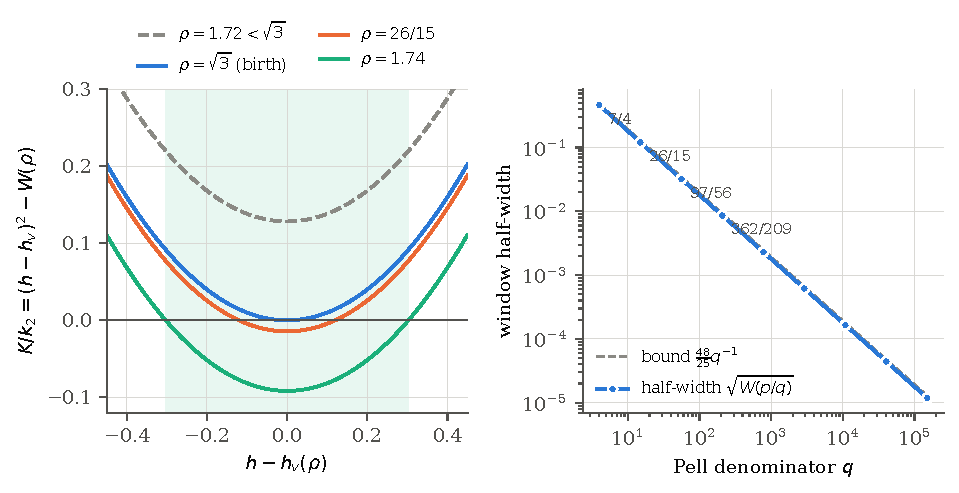
\includegraphics[width=\textwidth]{figures/window_geometry.pdf}
\caption{Left: $K/k_2=(h-h_v)^2-W$ against $h-h_v$ for $\rho\in\{1.72,\sqrt3,26/15,1.74\}$.
The four curves are vertical translates of one parabola. For $\rho<\sqrt3$ there is no
window; at $\rho=\sqrt3$ it is born as a double root; for $\rho>\sqrt3$ it is the interval
where the curve is negative, shaded for $\rho=1.74$. Right: the half-width $\sqrt W$ of the window at the Pell parameters $\rho=p/q$, against
$q$. It decays like $q^{-1}$. The dashed line is the bound $\tfrac{48}{25}q^{-1}$ implied
by Proposition~\ref{prop:cert}(c); it exceeds the actual half-width by less than $7\%$.}
\label{fig:window}
\end{figure}

Take $T=2$, so $N_0=16$ and the Pell search stops at $(p,q)=(97,56)$. Then
\[
\rho=\tfrac{97}{56},\quad \gamma=\tfrac{103}{14},\quad h_v=\tfrac{22259}{5644},\quad
h_0=\tfrac{25081}{5644},\quad \lambda=\tfrac14 .
\]
The window is the open interval
\[
\Bigl(\tfrac{133}{34},\,\tfrac{330}{83}\Bigr)=\Bigl(h_v-\tfrac{181}{5644},\ h_v+\tfrac{181}{5644}\Bigr),
\]
of half-width $181/5644\approx0.032<\lambda/2$. The load points of the subset sums
$s\in\{0,\dots,4\}$ are $h_0-s/4$:
\[
\tfrac{25081}{5644},\quad \tfrac{11835}{2822},\quad \tfrac{22259}{5644},\quad \tfrac{5212}{1411},\quad \tfrac{19437}{5644} .
\]
Only $s=2$ gives a point inside the window, and it lies at the centre
(Figure~\ref{fig:reduction}). The integer version $M(w)=L\,A(w)$ has $L=31\,606\,400$.

\paragraph{No-instance.} For $w=(1,3)$ the subset sums are $\{0,1,3,4\}$, so the
$6\times6$ matrix $A(1,3)$ is D-stable by Theorem~\ref{thm:main}.

\paragraph{Yes-instance.} For $w=(1,1,2)$ the subset $S=\{3\}$, which consists of the
third weight $w_3=2$, sums to $T$. Theorem~\ref{thm:main} yields a destabilizing
scaling. A simpler one, found by hand following the mechanism of the proof, assigns:
\begin{itemize}
\item rate $1$ to the three inner coordinates;
\item rate $2\cdot10^5$ to the port and to the attachment of weight $2$;
\item rate $10^{-4}$ to the two attachments of weight $1$.
\end{itemize}
The characteristic polynomial of the scaled $7\times7$ rational matrix has exactly two
roots in the open right half-plane, certified by the exact Routh array. Numerically they
are $\approx2.0\cdot10^{-6}\pm2.24\,i$. The fast attachment and the fast port realize the
static load $\tfrac12$ at the window centre, while the slow attachments are nearly
invisible. The construction of Lemma~\ref{lem:realize}, executed literally, also produces
a certified destabilizing scaling, but with far more extreme rate ratios.

\begin{figure}[t]
\centering
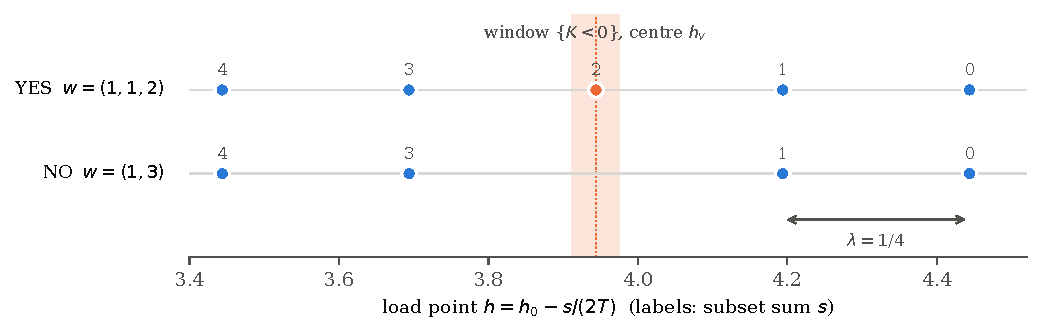
\includegraphics[width=\textwidth]{figures/reduction_example.pdf}
\caption{The worked example with $(p,q)=(97,56)$, $T=2$, $\lambda=\tfrac14$, on the axis
of the load point $h$. The shaded interval is the window $\{K<0\}$, of half-width
$181/5644$. Its centre $h_v$ is the load point of the subset sum $T$. Top: $w=(1,1,2)$; the sum $2$
lands at the centre, so the matrix is strictly D-unstable. Bottom: $w=(1,3)$; all sums
stay at distance $\ge\lambda$ from the centre, so the matrix is D-stable.}
\label{fig:reduction}
\end{figure}

% =========================================================================
\section{Formal verification}\label{sec:verification}

The development is in \texttt{proofs/DStabilityHardness/}. It is included, with every
module it imports, in the ancillary files of this article, under
\texttt{anc/lean/proofs/}. The paper-only root is \texttt{Paper.lean}. Its import closure
has $52$ modules including itself: the $13$ modules of Table~\ref{tab:lean} and $39$
library modules that they import directly or indirectly. It does not contain the modules
of the follow-up results mentioned below.
\begin{itemize}
\item It builds on verified libraries for the companion paper~\cite{companion2026},
namely absorption, reverse absorption, the safety theorem and spectral continuation,
and on a verified classification of positive-coefficient quartics.
\item It was compiled with Lean v4.30.0 and Mathlib at commit \lean{c5ea00351c28}, with
manifest hash \lean{a8df0b606ec2...}, treating warnings as errors. (This is the SHA-256
of the \texttt{lake-manifest.json} of the verification environment; the shipped manifest
differs only in the name of the root package.)
\item The exported declarations depend only on \lean{propext}, \lean{Classical.choice}
and \lean{Quot.sound}.
\item No \lean{sorry}, \lean{admit}, \lean{native_decide} or additional axiom occurs.
\end{itemize}
Positive diagonal scalings act on the right, $A\mapsto A\diag(d)$. D-stability, strict
D-instability and D-semistability have literal eigenpair semantics over $\C$: the
definitions \lean{DStable}, \lean{DUnstable} and \lean{DNonUnstable}.

\begin{table}[t]
\centering
\caption{Correspondence between the paper and the Lean development. File names are
relative to \texttt{anc/lean/proofs/}; ``companion'' abbreviates
\texttt{DStabilityCharacterization/}, ``hardness'' abbreviates
\texttt{DStabilityHardness/}, and ``quartic library'' is
\texttt{CollectiveInstability/QuarticClassification}.}
\label{tab:lean}
\small
\begin{tabular}{@{}>{\raggedright\arraybackslash}p{0.27\textwidth}>{\raggedright\arraybackslash}p{0.25\textwidth}>{\raggedright\arraybackslash}p{0.42\textwidth}@{}}\toprule
Result & File & Declaration(s)\\\midrule
Lemma~\ref{lem:quartic} & quartic library; hardness \texttt{Static} & \lean{matrix_hurwitzStable_of_delta_pos}, \lean{matrix_unstable_of_delta_neg}; \lean{quartic_axis_relations}\\
Lemma~\ref{lem:absorb} & companion \texttt{Granularity} & \lean{absorption}, \lean{load_bounds}, \lean{shift_pos}\\
Lemmas~\ref{lem:elim},~\ref{lem:reverse} & hardness \texttt{Window}; companion \texttt{FiniteRealization} & \lean{attached_pencil}, \lean{attached_static}, \lean{eigenpair_of_pencil}; \lean{reverse_absorption}\\
Theorem~\ref{thm:safety}, Lemma~\ref{lem:continuation} & companion \texttt{Granularity}, \texttt{SpectralContinuation} & \lean{attached_dStable_of_det}; \lean{hurwitzStable_on_preconnected}\\
\eqref{eq:coeffs}, $U\ge0$, Lemmas~\ref{lem:decomp},~\ref{lem:disc} & hardness \texttt{Family}, \texttt{Static}, \texttt{Window} & \lean{scaled_charpoly}, \lean{U_nonneg}, \lean{delta3_decomposition}, \lean{psi_decomposition}, \lean{Kf_quadratic}, \lean{k2_eq}, \lean{disc_factor}, \lean{Kf_vertex}, \lean{Kf_window}\\
Proposition~\ref{prop:cert} & hardness \texttt{Certificates}, \texttt{Symmetric}, \texttt{Static}, \texttt{Window} & \lean{F1_nonneg}, \lean{F2_nonneg}, \lean{Psi2_nonneg}; \lean{e2_pos}, \ldots, \lean{m4_pos}, \lean{F0_pos}; \lean{hv_bounds}, \lean{Wd_le}\\
Propositions~\ref{prop:static},~\ref{prop:contact} & hardness \texttt{Static} & \lean{static_dStable}, \lean{static_dUnstable}, \lean{contact_bound}\\
Lemma~\ref{lem:pell} & hardness \texttt{Reduction}, \texttt{Window}, \texttt{Paper} & \lean{pell_facts}, \lean{Wd_le}, \lean{Wd_base_neg}\\
Lemmas~\ref{lem:realize},~\ref{lem:rounding}; Proposition~\ref{prop:noaxis} & hardness \texttt{Reduction}, \texttt{Window} & \lean{subset_realization}; \lean{rounding_bound}; \lean{no_axis}\\
Theorem~\ref{thm:main} & hardness \texttt{Reduction}, \texttt{Main} & \lean{no_direction}, \lean{hardness_reduction}, \lean{hardness_iff}, \lean{dStability_partition_reduction}\\
Proposition~\ref{prop:encoding} & hardness \texttt{Encoding} & \lean{h0_formula}, \lean{hardIntMatrix_cast}, \lean{hardIntMatrix_bound}, \lean{pellSeq_pell}, \lean{pellSeq_three_pow}, \lean{pellSeq_p_le}, \lean{pellIndex_le_log}, \lean{pellIndex_q_le}\\
Scalar invariance; main theorem (promise form) & hardness \texttt{Encoding}, \texttt{Paper} & \lean{dStable_smul_iff}, \lean{dUnstable_smul_iff}; \lean{dStability_coNP_reduction}, \lean{partition_dichotomy}\\
\bottomrule\end{tabular}
\end{table}

\paragraph{How the certificates are checked.}
The three polynomials of Proposition~\ref{prop:cert}(b) are handled identically.
\begin{enumerate}
\item A script generates their homogenized forms as explicit Lean definitions, in blocks
of at most $24$ terms.
\item Lean proves, by \lean{ring}, that each function under the substitution equals its
form.
\item Writing every atom as a square, \lean{positivity} proves each block nonnegative.
\end{enumerate}
An eight-case sorting argument extends the ordered case to all nonnegative rates.

\paragraph{The formal main theorem.}
Let the weights $w$ be positive integers on a nonempty finite index type, with $\sum w=2T$.
The theorem \lean{partition_dichotomy} states the following. Let $N_0=\max(8T,4)$, let $k$ be the index
returned by \lean{pellIndex} for $N_0$, and let $(p,q)$ be the $k$-th term of
\lean{pellSeq}. Then:
\begin{itemize}
\item $k\le\lfloor\log_3N_0\rfloor+1$ and $q\le4N_0+1$;
\item every entry of the integer matrix \lean{hardIntMatrix}\,$p\,q\,w\,T$ is bounded by
$720q^3T$;
\item if no subset of $w$ sums to $T$, its real cast is D-stable and D-semistable;
\item if some subset sums to $T$, its real cast is strictly D-unstable, and neither
D-stable nor D-semistable.
\end{itemize}

\paragraph{What is not formal.}
\begin{itemize}
\item Remarks~\ref{rem:schur} and~\ref{rem:control}. They are not used in the proofs; their
computations are checked in exact arithmetic by \texttt{check\_paper.py}.
\item The complexity-theoretic packaging of Corollary~\ref{cor:complexity}: that the map is
computable in polynomial time, the handling of odd totals and of $m=0$, and the notion of
a Karp reduction. It follows from the explicit formulas, the entry bound and the
logarithmic Pell search, all of which are formal.
\end{itemize}
In complexity theory the running time of an explicit arithmetic map is usually checked
by inspection, as here. Mechanized complexity theory exists: Turing-machine programming
and the Cook--Levin theorem have been formalized in Coq~\cite{forster2020,gaher2021} and
in Isabelle~\cite{balbach2023}. Mathlib provides an interface for polynomial-time Turing
computability (\lean{Turing.TM2ComputableInPolyTime}), but even its closure under
composition is not yet proved there. A Lean proof of the running time of our reduction
would need, on top of that interface, a verified cost model for arithmetic on binary
integers. This is outside the scope of the present paper.

The receipt used for this paper verifies \texttt{Paper.lean}. One further declaration is
quoted in Section~\ref{sec:discussion}, open problem~3, and is not used in any proof:
\lean{destabilizing_port_fast}, in the module \texttt{TimeScale}. It is verified with a
second root, \texttt{All.lean}. Its import closure contains four modules beyond those of
\texttt{Paper.lean}, and it was checked with the same toolchain, Mathlib revision and
settings; the declaration depends on the same three axioms.

\paragraph{Exact computation.}
The script \texttt{check\_paper.py} in the ancillary files performs 42 checks. In exact
rational arithmetic it replays:
\begin{itemize}
\item the identities and certificates of Section~\ref{sec:core}, including the computations
of Remark~\ref{rem:schur} and the negative control of Remark~\ref{rem:control};
\item the Pell pairs and bounds, and the integer encoding;
\item every number of Section~\ref{sec:example}, with the exact Routh certificate of the
displayed destabilizing scaling;
\item the construction of Lemma~\ref{lem:realize}, executed literally on small
yes-instances and certified by exact Routh arrays.
\end{itemize}
It also checks that every shipped Lean source has the hash recorded in the verification
receipts, and it regenerates the certificate files \texttt{Certificates.lean} and
\texttt{CertificatesTimeScale.lean} byte for byte from the formulas of
Lemma~\ref{lem:decomp}. The script does not rerun Lean. Two checks are
floating-point sanity checks and are labelled as such: the $7\%$ statement of
Figure~\ref{fig:window} and the numerical value of the unstable pair in
Section~\ref{sec:example}.

% =========================================================================
\section{Related work and open problems}\label{sec:discussion}\label{sec:related}

\paragraph{Relation to known hardness results.}
\begin{itemize}
\item \emph{Structured singular values.} Chen, Fan and Yu~\cite{chen1995} related
D-stability to a condition on the real structured singular value $\mu$ of a matrix
built from $A$. Lee and Edgar~\cite{lee2001} gave the condition in the non-strict form
that characterizes D-stability; see~\cite{kushel2019} for this history. The recognition
problem for real $\mu$ is NP-hard~\cite{braatz1994}, but only for general matrices. The
hardness does not transfer to the special matrices arising from D-stability: a
reduction \emph{to} $\mu$ gives an upper bound, not a lower one.
\item \emph{Interval matrices.} Poljak and Rohn~\cite{poljak1993} and
Nemirovskii~\cite{nemirovskii1993} proved that deciding whether every member of an
interval matrix is nonsingular, respectively Hurwitz, is intractable; these universal
questions are coNP-hard in the terminology used here. In an interval family the entries
vary independently over a closed box. In the D-scaling family $\{\diag(d)A\}$ one
parameter scales a whole row, and the parameters range over an open cone; after
normalization this is the relative interior of a polytope whose vertices are singular
(see the next item). We are not aware of a reduction between the two kinds of family.
Structurally closest are two bordered constructions, like our star matrices.
Nemirovskii's result holds already when the uncertain entries lie in the last row and
column only~\cite{nemirovskii1993}; see also the survey~\cite{horacek2017}. Blondel and
Tsitsiklis~\cite{blondel1997} reduced PARTITION to the existence of a Hurwitz matrix in
an interval family whose uncertain entries also lie in the last row and column. Our
reduction is in the same spirit, but it must control arbitrarily large ratios between
the rates $d_i$ instead of entries in a closed box.
\item \emph{Matrix polytopes.} Gurvits and Olshevsky~\cite{gurvits2009} proved that
deciding whether every matrix in the convex hull of given matrices is Hurwitz is
intractable (again a coNP-hard universal question in our terminology).
Since D-stability is invariant under positive scalar multiples of $d$, $A$ is D-stable if
and only if every matrix in the relative interior of the polytope
$\operatorname{conv}\{\be_i\be_i^{\mathsf T}A: 1\le i\le N\}$ is Hurwitz. For $N\ge2$ the
generating matrices $\be_i\be_i^{\mathsf T}A$ have rank at most one and are never Hurwitz. So
D-stability concerns the relative interior of a very special polytope, and their result
does not imply ours.
\item \emph{P-matrices.} Coxson~\cite{coxson1994} proved that recognizing P-matrices is
coNP-complete. In the Hurwitz convention, D-stability implies that $-A$ is a
$P_0^+$-matrix~\cite{cross1978}, but the converse fails, so no reduction follows.
\end{itemize}
The survey of complexity results in systems and control by Blondel and
Tsitsiklis~\cite{blondel2000} does not treat D-stability. Our reduction exploits a
dynamical mechanism: the subset-sum obstruction
of the companion paper~\cite{companion2026}, made exact by the certificates of
Section~\ref{sec:core}.

\paragraph{Upper bounds and where the hardness lives.}
Strict D-instability asks for $d>0$ and $z$ with $\Real z>0$ and $\det(z-\diag(d)A)=0$. This
is a sentence of the existential theory of the reals. Likewise, D-stability and
D-semistability are negations of existential sentences. All three are therefore decidable
in polynomial space~\cite{canny1988,renegar1992a}.

For fixed order $N$ the number of variables is fixed. The problems are then decidable in
time polynomial in the bit length~\cite{renegar1992a,renegar1992b,renegar1992c,basu2006}, so, unless P${}={}$NP,
hardness requires growing dimension.

Our instances need entries of magnitude $\Theta(T^4)$ and exponentially fine windows.
Accordingly, the hardness is weak: with unary weights, $T$ is polynomial and PARTITION is
easy.

\paragraph{Open problems.}
\begin{enumerate}[leftmargin=1.6em]
\item \emph{Strong hardness.} Is D-stability coNP-hard for matrices whose entries have
polynomially bounded numerators and denominators? A natural route combines several ports,
each carrying its own window.
\item \emph{Membership and exact complexity.} Is D-semistability in coNP? Equivalently, is
strict D-instability in NP? This would follow, for instance, if every strictly D-unstable
rational matrix had a destabilizing scaling of polynomial bit length. At the other end,
are these problems $\exists\R$-hard?
\item \emph{Bounded heterogeneity.} The destabilizing scalings in the proof of
Theorem~\ref{thm:main}\,(i) use rate ratios that grow with $T$. In the proof the port is
faster than the inner coordinates by a factor of order $|K|^{-1}=\Theta(q^2)$ (proof of
Proposition~\ref{prop:static}), and the attachment rates of Lemma~\ref{lem:realize} are
more extreme still. This is unavoidable for our matrices: every positive scaling of
$A(w)$ with an eigenvalue in the closed right half-plane has port rate larger than $q^2$
times the sum of the three inner rates. (This is the Lean declaration
\lean{destabilizing_port_fast}, see Section~\ref{sec:verification}; it is not used in our
proofs.) The port rate is at most $\max_id_i$ and the sum of the inner rates is at least
$3\min_id_i$, so such a scaling has $\max_id_i/\min_id_i>3q^2$. Hence, once $3q^2\ge R$,
every positive scaling of $A(w)$ with $\max_id_i/\min_id_i\le R$ is Hurwitz, whatever the
answer to the PARTITION instance, and the reduction says nothing about bounded
heterogeneity. Is D-stability restricted to scalings with $\max_id_i/\min_id_i\le R$
still hard for fixed $R$?
\end{enumerate}

\section*{Data and code availability}
The ancillary files of this article (directory \texttt{anc/}) contain:
\begin{itemize}
\item the Lean sources of both roots and of every module they import, with the toolchain
pin, the Mathlib manifest and a \texttt{lakefile.lean};
\item summaries of the two verification receipts, listing the SHA-256 hash of every source
file and the axioms of the exported declarations;
\item the exact replay script \texttt{check\_paper.py} with its helper module, and the
generator of the certificate files;
\item a \texttt{README.md} with the verification commands.
\end{itemize}

\bibliographystyle{plainurl}
\bibliography{refs}

\end{document}
